\documentclass[12pt,a4paper]{article}
\usepackage{tikz}
\begin{document}
	\begin{enumerate}
		\item Assume that the minimum page size, such that the entire page table fits well in one page is $x$, we have $2^{28} \div x \times 4 = x$, thus $x = 2^{15}$. So the page size is $32$KB.
		
		\item 
			\begin{enumerate}
				\item[1)] If we use \emph{First Fit Algorithm}, the fourth process have to wait until the system have a large enough hole to hold it. Thus, we have \\
					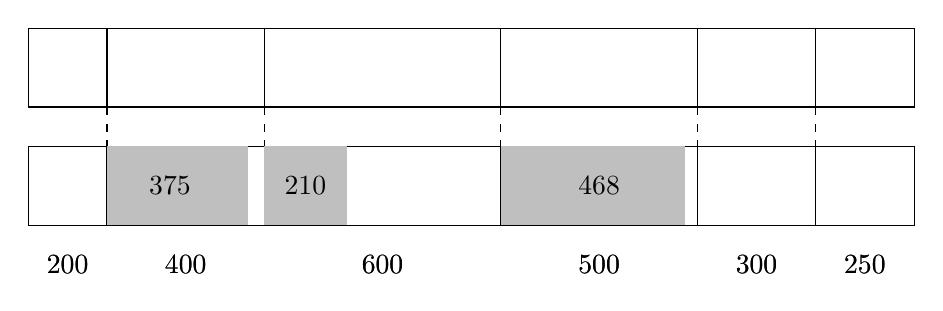
\begin{tikzpicture}
						\draw (0,1.5) rectangle (11.25,2.5);
						\draw (1,1.5) -- (1,2.5);
						\draw (3,1.5) -- (3,2.5);
						\draw (6,1.5) -- (6,2.5);
						\draw (8.5,1.5) -- (8.5,2.5);
						\draw (10,1.5) -- (10,2.5);
						\path (0.5,-0.5) node  {$200$};
						\path (2,-0.5) node  {$400$};
						\path (4.5,-0.5) node  {$600$};
						\path (7.25,-0.5) node  {$500$};
						\path (9.25,-0.5) node  {$300$};
						\path (10.625,-0.5) node  {$250$};
						
						\draw[dashed] (1,1.5) -- (1,1);
						\draw[dashed] (3,1.5) -- (3,1);
						\draw[dashed] (6,1.5) -- (6,1);
						\draw[dashed] (8.5,1.5) -- (8.5,1);
						\draw[dashed] (10,1.5) -- (10,1);
						
						\draw (0,0) rectangle (11.25,1);
						\draw (1,0) -- (1,1);
						\draw (3,0) -- (3,1);
						\draw (6,0) -- (6,1);
						\draw (8.5,0) -- (8.5,1);
						\draw (10,0) -- (10,1);
						\path (0.5,-0.5) node  {$200$};
						\path (2,-0.5) node  {$400$};
						\path (4.5,-0.5) node  {$600$};
						\path (7.25,-0.5) node  {$500$};
						\path (9.25,-0.5) node  {$300$};
						\path (10.625,-0.5) node  {$250$};
						\fill[color = gray!50] (1,0) rectangle (2.785,1);
						\fill[color = gray!50] (3,0) rectangle (4.05,1);
						\fill[color = gray!50] (6,0) rectangle (8.34,1);
						
						\path (1.8,0.5) node  {$375$};
						\path (3.52,0.5) node  {$210$};
						\path (7.25,0.5) node  {$468$};
					\end{tikzpicture}
					
				\item[2)] If we use \emph{Best Fit Algorithm}, we have\\
					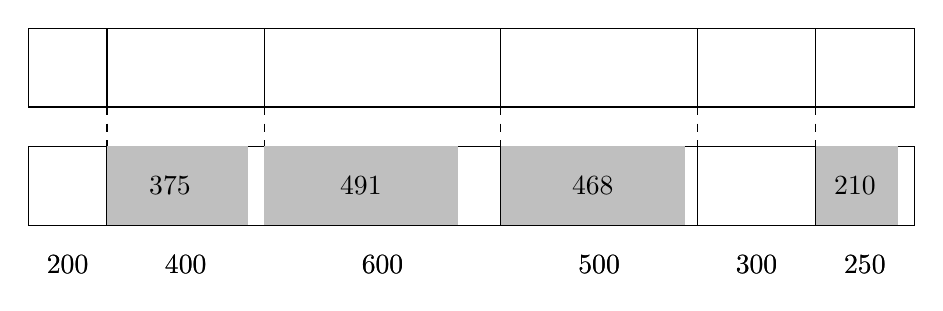
\begin{tikzpicture}
					\draw (0,1.5) rectangle (11.25,2.5);
					\draw (1,1.5) -- (1,2.5);
					\draw (3,1.5) -- (3,2.5);
					\draw (6,1.5) -- (6,2.5);
					\draw (8.5,1.5) -- (8.5,2.5);
					\draw (10,1.5) -- (10,2.5);
					\path (0.5,-0.5) node  {$200$};
					\path (2,-0.5) node  {$400$};
					\path (4.5,-0.5) node  {$600$};
					\path (7.25,-0.5) node  {$500$};
					\path (9.25,-0.5) node  {$300$};
					\path (10.625,-0.5) node  {$250$};
					
					\draw[dashed] (1,1.5) -- (1,1);
					\draw[dashed] (3,1.5) -- (3,1);
					\draw[dashed] (6,1.5) -- (6,1);
					\draw[dashed] (8.5,1.5) -- (8.5,1);
					\draw[dashed] (10,1.5) -- (10,1);
					
					\draw (0,0) rectangle (11.25,1);
					\draw (1,0) -- (1,1);
					\draw (3,0) -- (3,1);
					\draw (6,0) -- (6,1);
					\draw (8.5,0) -- (8.5,1);
					\draw (10,0) -- (10,1);
					\path (0.5,-0.5) node  {$200$};
					\path (2,-0.5) node  {$400$};
					\path (4.5,-0.5) node  {$600$};
					\path (7.25,-0.5) node  {$500$};
					\path (9.25,-0.5) node  {$300$};
					\path (10.625,-0.5) node  {$250$};
					
					\fill[color = gray!50] (1,0) rectangle (2.785,1);
					\path (1.8,0.5) node  {$375$};
					\fill[color = gray!50] (10,0) rectangle (11.05,1);
					\path (10.5,0.5) node  {$210$};
					\fill[color = gray!50] (6,0) rectangle (8.34,1);
					\path (7.17,0.5) node  {$468$};
					\fill[color = gray!50] (3,0) rectangle (5.455,1);
					\path (4.225,0.5) node  {$491$};
					\end{tikzpicture}
					
				\item[3)] If we use \emph{Worst Fit Algorithm}, the third and fourth processes need to wait until the system has large enough holes to hold them. Thus, we have \\
					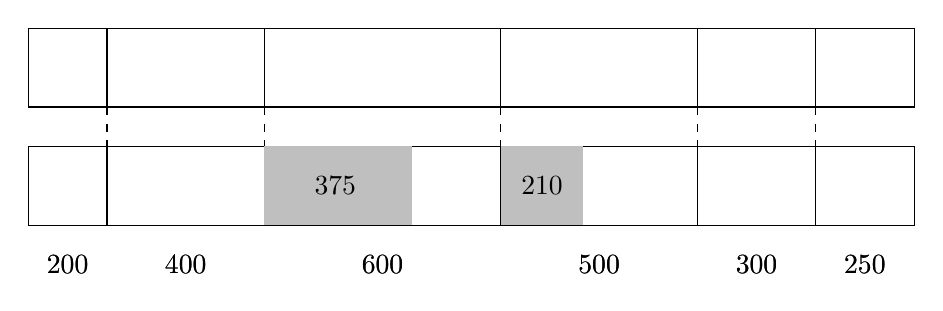
\begin{tikzpicture}
					\draw (0,1.5) rectangle (11.25,2.5);
					\draw (1,1.5) -- (1,2.5);
					\draw (3,1.5) -- (3,2.5);
					\draw (6,1.5) -- (6,2.5);
					\draw (8.5,1.5) -- (8.5,2.5);
					\draw (10,1.5) -- (10,2.5);
					\path (0.5,-0.5) node  {$200$};
					\path (2,-0.5) node  {$400$};
					\path (4.5,-0.5) node  {$600$};
					\path (7.25,-0.5) node  {$500$};
					\path (9.25,-0.5) node  {$300$};
					\path (10.625,-0.5) node  {$250$};
					
					\draw[dashed] (1,1.5) -- (1,1);
					\draw[dashed] (3,1.5) -- (3,1);
					\draw[dashed] (6,1.5) -- (6,1);
					\draw[dashed] (8.5,1.5) -- (8.5,1);
					\draw[dashed] (10,1.5) -- (10,1);
					
					\draw (0,0) rectangle (11.25,1);
					\draw (1,0) -- (1,1);
					\draw (3,0) -- (3,1);
					\draw (6,0) -- (6,1);
					\draw (8.5,0) -- (8.5,1);
					\draw (10,0) -- (10,1);
					\path (0.5,-0.5) node  {$200$};
					\path (2,-0.5) node  {$400$};
					\path (4.5,-0.5) node  {$600$};
					\path (7.25,-0.5) node  {$500$};
					\path (9.25,-0.5) node  {$300$};
					\path (10.625,-0.5) node  {$250$};
					
					\fill[color = gray!50] (3,0) rectangle (4.875,1);
					\path (3.9,0.5) node  {$375$};
					\fill[color = gray!50] (6,0) rectangle (7.05,1);
					\path (6.525,0.5) node  {$210$};
					\end{tikzpicture}
			\end{enumerate}
		\item 
			\begin{enumerate}
				\item[1)] Since the	memory is byte addressable and virtual address is 64 bits long, so the virtual address space is $2^{64}$ bytes. One page can hold $2^{20}/2^{2} = 2^{18}$ page table entries. If we use $2$ levels of page table, then we can only cover $2^{18} \times 2^{18} \times 20^{20} = 2^{56}$ bytes of space, if we use $3$ levels of page table, we will be able to cover $2^{18} \times 2^{18} \times 2^{18} \times 2^{20} = 2^{74}$ bytes. Thus, we need $3$ levels of page table.
				
				\item[2)] The struct of virtual address is like below \\
					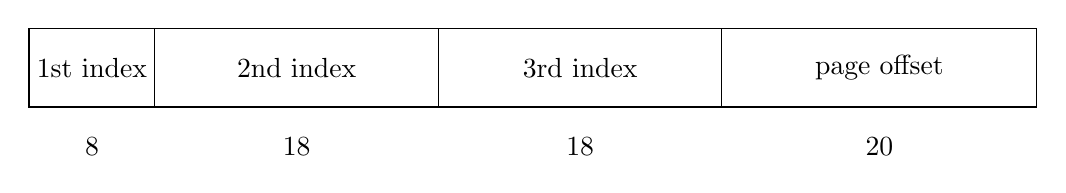
\begin{tikzpicture}
						\draw (0,0) rectangle (12.8,1);
						\draw (1.6,0) -- (1.6,1);
						\draw (5.2,0) -- (5.2,1);
						\draw (8.8,0) -- (8.8,1);
						\path (0.8,-0.5) node  {$8$};
						\path (3.4,-0.5) node  {$18$};
						\path (7,-0.5) node  {$18$};
						\path (10.8,-0.5) node  {$20$};
						
						\path (0.8,0.5) node  {$1\textrm{st index}$};
						\path (3.4,0.5) node  {$2\textrm{nd index}$};
						\path (7,0.5) node  {$3\textrm{rd index}$};
						\path (10.8,0.5) node  {$\textrm{page offset}$};
					\end{tikzpicture}
					The struct of physical address is like below \\
						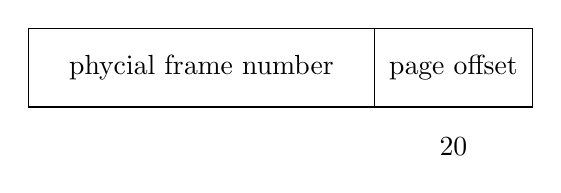
\begin{tikzpicture}
						\draw (0,0) rectangle (6.4,1);
						\draw (4.4,0) -- (4.4,1);
						\path (5.4,-0.5) node  {$20$};
						
						\path (2.2,0.5) node  {$\textrm{phycial frame number}$};
						\path (5.4,0.5) node  {$\textrm{page offset}$};
						\end{tikzpicture}
			\end{enumerate}
		
		\item 
			\begin{enumerate}
				\item[1)] The total number of page faults is $6$, hit ratio is $40\%$ and miss ratio is $60\%$.
				
				\item[2)] The total number of page faults is $6$, hit ratio is $40\%$ and miss ratio is $60\%$.
				
				\item[3)] The total number of page faults is $5$, hit ratio is $50\%$ and miss ratio is $50\%$.
			\end{enumerate}
		
		\item $EAT = (100+20) \times 0.8 + (200+20) \times 0.2 = 140$ns.
		
		\item 
			\begin{itemize}
				\item FCFS: $$(100 - 23) + (89 - 23) + (132 - 89) + (132 - 42) + (187 - 42) = 421.$$
				\item SSTF: $$(100 - 89) + (132 - 89) + (187 - 132) + (187 - 42) + (42 - 23) = 273.$$
				\item SCAN: $$(100 - 89) + (89 - 42) + (42 - 23) + (23 - 0) + (132 - 0) + (187 - 132) = 287.$$
				\item C-SCAN: $$(100 - 89) + (89 - 42) + (42 - 23) + (23 - 0) + (199 - 0) + (199 - 187) + (187 - 132) = 366.$$
				\item C-LOOK: $$(100 - 89) + (89 - 42) + (42 - 23) + (187 - 0) + (187 - 132) = 319.$$
			\end{itemize}
	\end{enumerate}
\end{document}